\documentclass[usenames,dvipsnames,10pt]{beamer}

\usetheme{Copenhagen}

\usepackage{tikz}
\usepackage{tkz-berge}
\usepackage{tkz-graph}
\usepackage{subcaption}
\usepackage{blkarray}
\usepackage{aligned-overset}
\usepackage{graphicx}
\usepackage{calc}

\setbeamertemplate{footline}[frame number]

\usetikzlibrary{patterns,arrows,decorations.pathreplacing}

\usepackage{xcolor}
\definecolor{dblue}{RGB}{20,66,129}
\definecolor{rose}{RGB}{255,101,122}
\definecolor{crimsonred}{RGB}{132,22,23}
\definecolor{darkblue}{RGB}{72,61,139}

\definecolor{deepblue}{RGB}{36,123,160}
\definecolor{deepred}{RGB}{255,22,84}
\definecolor{deeporange}{RGB}{240,111,62}

\definecolor{olive}{rgb}{0.3, 0.4, .1}
\definecolor{fore}{RGB}{249,242,215}
\definecolor{back}{RGB}{51,51,51}
\definecolor{title}{RGB}{255,0,90}
\definecolor{dgreen}{rgb}{0.,0.6,0.}
\definecolor{gold}{rgb}{1.,0.84,0.}
\definecolor{JungleGreen}{cmyk}{0.99,0,0.52,0}
\definecolor{BlueGreen}{cmyk}{0.85,0,0.33,0}
\definecolor{RawSienna}{cmyk}{0,0.72,1,0.45}
\definecolor{Magenta}{cmyk}{0,1,0,0}

\DeclareMathOperator{\QQ}{\mathbb{Q}}
\DeclareMathOperator{\ZZ}{\mathbb{Z}}
\DeclareMathOperator{\RR}{\mathbb{R}}
\DeclareMathOperator{\HH}{\mathbb{H}}
\DeclareMathOperator{\CC}{\mathbb{C}}
\DeclareMathOperator{\AB}{\mathbb{A}}
\DeclareMathOperator{\PP}{\mathbb{P}}
\DeclareMathOperator{\MM}{\mathbf{M}}
\DeclareMathOperator{\VV}{\mathbf{V}}
\DeclareMathOperator{\TT}{\mathbf{T}}
\DeclareMathOperator{\LL}{\mathcal{L}}
\DeclareMathOperator{\EE}{\mathbb{E}}
\DeclareMathOperator{\NN}{\mathbf{N}}
\DeclareMathOperator{\DQ}{\mathcal{Q}}
\DeclareMathOperator{\IA}{\mathfrak{a}}
\DeclareMathOperator{\IB}{\mathfrak{b}}
\DeclareMathOperator{\IC}{\mathfrak{c}}
\DeclareMathOperator{\IP}{\mathfrak{p}}
\DeclareMathOperator{\IQ}{\mathfrak{q}}
\DeclareMathOperator{\IM}{\mathfrak{m}}
\DeclareMathOperator{\IN}{\mathfrak{n}}
\DeclareMathOperator{\IK}{\mathfrak{k}}
\DeclareMathOperator{\ord}{\text{ord}}
\DeclareMathOperator{\Ker}{\textsf{Ker}}
\DeclareMathOperator{\Coker}{\textsf{Coker}}
\DeclareMathOperator{\emphcoker}{\emph{coker}}
\DeclareMathOperator{\pp}{\partial}
\DeclareMathOperator{\tr}{\text{tr}}

\newtheorem*{goal}{Fourier Multipliers on $\RR^d$}
\newtheorem*{goall}{Spectral Multipliers on $S^d$}

\newtheorem*{mainquestion}{Main Question}
\AtBeginEnvironment{mainquestion}{%
  \setbeamercolor{block title}{use=example text,fg=black,bg=yellow!75!black}
  \setbeamercolor{block body}{parent=normal text,use=block title example,bg=yellow!10}
}

\newtheorem*{nothing}{}
\newtheorem*{superconjecture}{The Radial Multiplier (Super) Conjecture}
\newtheorem*{partialsums}{$L^p$ Convergence of Partial Sums}



\title{A Characterization of $L^p$ Boundedness For Non-Compactly Supported Multipliers of Spherical Harmonic Expansions}
\author{Jacob Denson}

\institute{University of Wisconsin Madison}

\begin{document}

\maketitle

\begin{frame}

    % Write Notation on Board
    \begin{goal}
        Given $m: [0,\infty) \to \CC$, define an operator $F_m$ on $\RR^d$ by setting
        %
        \[ (F_m g)(x) = \int_{\RR^d} m(|\xi|) \widehat{g}(\xi) e^{2 \pi i \xi \cdot x}\; d \xi. \]
    \end{goal}

    \pause

    \begin{goall}
        Every $f: S^d \to \CC$ has a spherical harmonic expansion $f = \sum_{k = 0}^\infty f_k$, where $f_k$ is a homogeneous harmonic polynomial on $\RR^{d+1}$ of degree $k$.\vspace{0.5em}

        Given $m: [0,\infty) \to \CC$, define
        %
        \[ T_m f = \sum\nolimits_{k = 0}^\infty m(k) f_k. \]
    \end{goall}

    \pause

    \begin{mainquestion}
        Can methods for obtaining $L^p$ bounds for Fourier multiplier operators be extended to obtain $L^p$ bounds for spectral multiplier operators.
    \end{mainquestion}

%        \item Let $(M^d,g)$ be a compact Riemannian manifold.
%        \item Let $e_\lambda \in C^\infty(M)$, $\Delta_g e_\lambda = - \lambda^2 e_\lambda$.
%        \item \emph{Nodal Set} of $e_\lambda$: $Z_\lambda = \{ x \in M: e_\lambda(x) = 0 \}$.
%        \item \emph{Nodal Domain} $D_\lambda$: a connected component of $M - Z_\lambda$.

        % TODO: Add Pictures

        % lambda = sqrt(l(l+1))
        % Separation of Variables: e_lambda(theta,psi) = Theta(theta) Phi(phi)
        
        % Zonal Harmonic: P_l(cos theta). Zeroes are roughly spaced at a distance O(1/l) = O(1/lambda) apart.
        % Roots of P_l are approximately (1 - 1/8n^2) cos(pi k/n)

        % Also spaced a distance O(1/lambda) apart

        % Tesseral: P^m_l(cos theta) cos(m phi)
        % |m| <= lambda
        % Again, observe O(1/lambda) thickness boxes.
\end{frame}

\begin{frame}
    \begin{mainquestion}
        Can methods for obtaining $L^p$ bounds for Fourier multiplier operators be extended to obtain $L^p$ bounds for spectral multiplier operators.
    \end{mainquestion}

    \begin{itemize}
        \pause
        \item Roughly speaking, $F_m = \lim_{R \to \infty} T_{m_R}$,  where $m_R(t) = m(t / R)$, because dilating the multiplier can be understood as \emph{dilating the metric} on $S^d$. Thus
        %
        \[ \| F_m \|_{L^p(\RR^d) \to L^p(\RR^d)} \lesssim \limsup_{R \to \infty} \| T_{m_R} \|_{L^p(S^d) \to L^p(S^d)}. \]
        %
        Thus problems about operators on manifolds invariant under dilation are \emph{always harder}.

        \pause
        \item Heuristic: High frequency behaviour on a manifold can be understood by methods akin to Euclidean settings.

        \pause
        \item However, some phenomena are not the same, and it remains mysterious \emph{when} and \emph{why} this is the case.
    \end{itemize}
\end{frame}

\begin{frame}
    \small
    \begin{superconjecture}
        If $a(\xi) = m(|\xi|)$ is compactly supported, and $1 < p < \frac{2d}{d+1}$, then
        %
        \[ \| F_m \|_{L^p(\RR^d) \to L^p(\RR^d)} \sim \| \widehat{a}\; \|_{L^p(\RR^d)}. \]
        %
        \pause
        In general, if $a(\xi) = \sum_{k = -\infty}^\infty a_k(\xi / 2^k)$, where $a_k(\xi) = m_k(|\xi|)$, then
        %
        \[ \| F_a \|_{L^p(\RR^d) \to L^p(\RR^d)} \sim \sup\nolimits_k \| \widehat{a}_k \|_{L^p(\RR^d)}. \]
        %
        \pause
        Note that if $a$ is compactly supported, then
        %
        \[ \| \widehat{a} \|_{L^p(\RR^d)} \sim \left( \int_0^\infty |\widehat{m}(t)|^p \langle t \rangle^{(d-1)(1 - p/2)} \right)^{1/p}. \]
    \end{superconjecture}
    \normalsize

    \begin{itemize}
        \pause
        \item (Heo, Nazarov, Seeger) True if $1 < p < \frac{2(d-1)}{d+1}$.

        \item (Cladek) True when $p = 3$ and $1 < p < 13/12$, and when $p = 4$ and $1 < p < 36/29$, for \emph{compactly supported} $a$.
    \end{itemize}

    \pause
    \begin{nothing}
        There are reasons to believe that analogues of the super conjecture fail in the full range on an arbitrary compact manifold. But the sphere is \emph{likely safe} (constant curvature).
    \end{nothing}
\end{frame}

\begin{frame}
    \frametitle{Main Theorem}

    \small
    \begin{theorem}
        If $1 < p < \frac{2(d-1)}{d+1}$, then for all $m: [0,\infty) \to \RR$, if $m = \sum m_k(\cdot/2^k)$, then
        %
        \[ \| T_m \|_{L^p(S^d) \to L^p(S^d)} \lesssim \sup\nolimits_k \left( \int_0^\infty |\widehat{m}_k(t)|^p \langle t \rangle^{(d-1)(1 - p/2)} \right)^{1/p} \]
        %
        and
        %
        \[ \sup\nolimits_R \| T_{m_R} \|_{L^p(S^d) \to L^p(S^d)} \sim \sup\nolimits_k \left( \int_0^\infty |\widehat{m}_k(t)|^p \langle t \rangle^{(d-1)(1 - p/2)} \right)^{1/p}. \]
    \end{theorem}

    \pause

    \begin{partialsums}
        If $1 < p < \frac{2(d-1)}{d+1}$, then for all $m: [0,\infty) \to \RR$,
        %
        \[ \lim_{R \to \infty} \sum\nolimits_{k = 0}^\infty m(k/R) f_k = f \quad\text{for all $f \in L^p(S^d)$} \]
        %
        if and only if $m(0) = 1$ and $\sup\nolimits_k \left( \int_0^\infty |\widehat{m}_k(t)|^p \langle t \rangle^{(d-1)(1 - p/2)} \right)^{1/p} < \infty$.
    \end{partialsums}
    \normalsize
\end{frame}

\begin{frame}
    \frametitle{Combining Dyadic Scales}

    \small
    \begin{theorem}
        Suppose $1 < p_0 < \frac{2d}{d+1}$, and that
        %
        \scriptsize
        \begin{align*}
            \left\| \sum\nolimits_{(x_0,t_0) \in \mathcal{X}_k \times \mathcal{T}_k} c(x_0,t_0) [P_k \circ W_t](\cdot,x_0) \right\|_{L^p(S^d)} \lesssim 2^{k \frac{d+1}{p}} \left( \sum |c(x_0,t_0)|^p \langle 2^k t_0 \rangle^{(d-1)(1 - p/2)} \right)^{1/p}.
        \end{align*}
        \normalsize
        %
        holds uniformly in $k$, where $\mathcal{X}_k$ and $\mathcal{T}_k$ are maximal $2^{-k}$ separated subsets of $M$ and $[0,\infty)$ respectively. Then for $1 \leq p < p_0$,
        %
        \[ \| T_m \|_{L^p(S^d) \to L^p(S^d)} \lesssim \sup\nolimits_k \left( \int_0^\infty |\widehat{m}_k(t)|^p \langle t \rangle^{(d-1)(1 - p/2)} \right)^{1/p}. \]
    \end{theorem}

    \pause
    \begin{nothing}
        If $T = T_m$ and $T_k = T_{m_k}$, the Theorem is about bounding $T = \sum T_k$ under uniform control over the operators $\{ T_k \}$. Assumption naturally arises when controlling $T_k$ using the wave representation of $T_k$, i.e. for any $m$,
        %
        \[ T_{m} = \int_0^\infty \widehat{m}(t) W(t)\; dt. \]
    \end{nothing}
    \normalsize
\end{frame}

\begin{frame}
    \frametitle{Method: $L^p$ Atomic Decomposition}

    \begin{itemize}
        \item How do we control the interaction between different frequency scales?

        \pause
        \item Given $f \in L^p(S^d)$, if we consider `Littlewood-Paley projections' $P_k$, then we have a Littlewood-Paley type square function estimate
        %
        \[ \left\| \left( \sum |f_k|^2 \right)^{1/2} \right\|_{L^p(S^d)} \lesssim \| f \|_{L^p(S^d)}. \]

        \pause
        \item On it's own, this is not enough. Need more `spatial control' on the operator $T$. Obtain this by using an `atomic decomposition in $L^p$'.
    \end{itemize}
\end{frame}

\begin{frame}
    \frametitle{Method: $L^p$ Atomic Decomposition}

    \small
    \begin{itemize}
        \item For simplicity, suppose that
        %
        \[ \left( \sum\nolimits_{k \in \ZZ} |f_k|^2 \right)^{1/2} \sim 1 \]
        %
        on a set $\Omega \subset S^d$, and is negligible elsewhere.

        \pause
        \item Goal: Show that
        %
        \[ \| T_mf \|_{L^p(S^d)} \lesssim |\Omega|^{1/p}. \]

        \pause
        \item Consider a Whitney decomposition $\Omega = \bigcup W$. Then we can write $f = \sum_{k,W} a_{k,W}$, where $a_{k,W}$ is `frequency $2^k$', supported on $W$, and, morally speaking, if $H = \| a_{k,W} \|_{L^\infty(S^d)}$, then $\| a_{k,W} \|_{L^p(S^d)} \sim H |W|^{1/p}$.
        %
%        \[ \| a_{k,W} \|_{L^p(S^d)} \lesssim \| a_{k,W} \|_{L^\infty(S^d)} |W|^{1/p}. \]
    \end{itemize}
    \pause

    \centering
    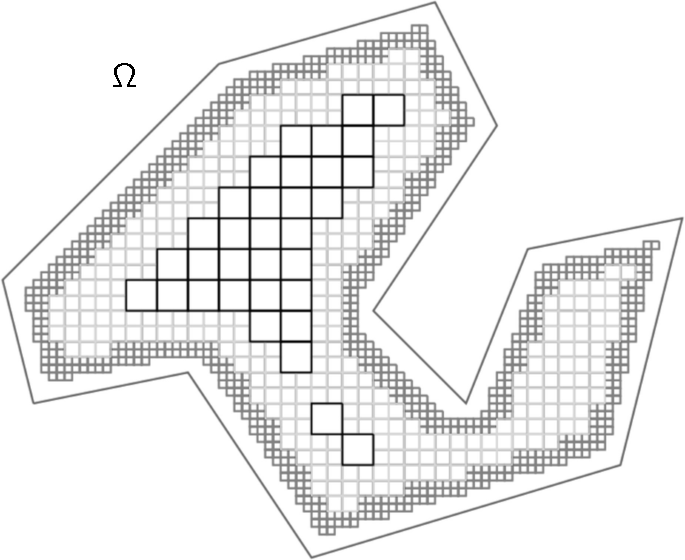
\includegraphics[width=5cm]{449605_1_En_6_Fig1_HTML.png}
\end{frame}


\begin{frame}
    \frametitle{Short and Long Range Interactions}

    \begin{itemize}
        \item Fourier Inversion Formula:
        %
        \[ Ta_{k,W} = \int_0^\infty \widehat{m}_k(t) (P_k \circ W_t) \{ a_{k,W} \}\; dt \]
        \pause

        \item Write $Ta_{k,W} = \text{Short}_{k,W} + \text{Long}_{k,W}$, where
        %
        \[ \text{Short}_{k,W} = \int_0^{l(W)}\widehat{m}_k(t) (P_k \circ W_t) \{ a_{k,W} \} \]
        %
        and
        %
        \[ \text{Long}_{k,W} = \int_{l(W)}^\infty \widehat{m}_k(t) (P_k \circ W_t) \{ a_{k,W} \}. \]
    \end{itemize}
\end{frame}




\begin{frame}
    \frametitle{Short Range Interactions}

    The support of $\text{Short}_{k,W}$ is contained in $W^*$.
    \vspace{1em}

    \pause
    Since the sets $\{ W^* \}$ have the bounded overlap property, we can use almost orthogonality to conclude that
        %
        \begin{align*}
            \left\| \sum\nolimits_{k,W} \text{Short}_{k,W} \right\|_{L^2(S^d)} &\lesssim \left( \sum\nolimits_{k,W} \| \text{Short}_{k,W} \|_{L^2(S^d)}^2 \right)^{1/2}
        \end{align*}
        %
        \pause 
        Roughly speaking, $\text{Short}_{k,W} \approx T_k a_{k,W}$ (or at least a smoothening of it), so
        %
        \begin{align*}
            \left( \sum\nolimits_{k,W} \| \text{Short}_{k,W} \|_{L^2(S^d)}^2 \right)^{1/2} &\lesssim \left( \sum \nolimits_{k,W} \| a_{k,W} \|_{L^2(S^d)}^2 \right)^{1/2}\\
            &\lesssim \left\| \left( \sum |a_{k,W}|^2 \right)^{1/2} \right\|_{L^2(S^d)}\\
            &\lesssim |\Omega|^{1/2}.
        \end{align*}
        %
        \pause 
        H\"{o}lder's inequality implies $\| \sum\nolimits_{k,W} \text{Short}_{k,W} \|_{L^p(S^d)} \lesssim |\Omega|^{1/p}$.
\end{frame}


\begin{frame}
    \frametitle{Long Range Interactions}

    Long range interactions exhibit exponential decay, i.e. for each $k$, our assumption implies that for $1 \leq p < p_0$,
    %
    \[ \left\| \sum\nolimits_{l(W) = l - k} \text{Long}_{k,W} \right\|_{L^p(S^d)} \lesssim 2^{-l \varepsilon} \left( \sum\nolimits_{l(W) = l-k} |W| \| a_{k,W} \|_{L^\infty(S^d)}^p \right)^{1/p}. \]
    %
    \pause
    But then by $L^2$ orthogonality,
    %
    \small
    \begin{align*}
        \left\| \sum\nolimits_k \sum\nolimits_{l(W) = l - k} \text{Long}_{k,W} \right\|_{L^p(S^d)} &\lesssim \left( \sum\nolimits_k \left\| \sum\nolimits_{l(W) = l-k} \text{Long}_{k,W} \right\|_{L^p(S^d)}^p \right)^{1/p}\\
        &\lesssim 2^{-l \varepsilon} \left( \sum\nolimits_k \sum\nolimits_{l(W) = l - k} |W| \| a_{k,W} \|_{L^\infty(S^d)}^p \right)^{1/p}.
    \end{align*}
    \normalsize
    %
    Now we have no more interactions in space, i.e.
    %
    \[ \left( \sum\nolimits_k \sum\nolimits_{l(W) = l - k} |W| \| a_{k,W} \|_{L^\infty(S^d)}^p \right)^{1/p} \lesssim |\Omega|^{1/p}. \]
    %
    \pause 
    We win if we sum in $l$ using the triangle inequality.
\end{frame}


\begin{frame}
    \frametitle{Thanks For Listening!}

    \small
    \begin{theorem}
        If $1 < p < \frac{2(d-1)}{d+1}$, then for all $m: [0,\infty) \to \RR$, if $m = \sum m_k(\cdot/2^k)$, then
        %
        \[ \| T_m \|_{L^p(S^d) \to L^p(S^d)} \lesssim \sup\nolimits_k \left( \int_0^\infty |\widehat{m}_k(t)|^p \langle t \rangle^{(d-1)(1 - p/2)} \right)^{1/p}. \]
    \end{theorem}

    \begin{theorem}
        Suppose $1 < p_0 < \frac{2d}{d+1}$, and that the bound
        %
        \[ \left\| \sum_{(x_0,t_0) \in \mathcal{X}_k \times \mathcal{T}_k} c(x_0,t_0) [P_k \circ W_t] \right\|_{L^p(S^d)} \lesssim \left( \sum |c(x_0,t_0)|^p \langle 2^k t_0 \rangle^{(d-1)(1 - p/2)} \right)^{1/p}. \]
        %
        holds uniformly in $k$, where $\mathcal{X}_k$ and $\mathcal{T}_k$ are maximal $2^{-k}$ separated subsets of $M$ and $[0,\infty)$ respectively. Then for $1 \leq p < p_0$,
        %
        \[ \| T_m \|_{L^p(S^d) \to L^p(S^d)} \lesssim \sup\nolimits_k \left( \int_0^\infty |\widehat{m}_k(t)|^p \langle t \rangle^{(d-1)(1 - p/2)} \right)^{1/p}. \]
    \end{theorem}
    \normalsize
\end{frame}

\end{document}